\documentclass[tikz,border=10pt]{standalone}

\begin{document}
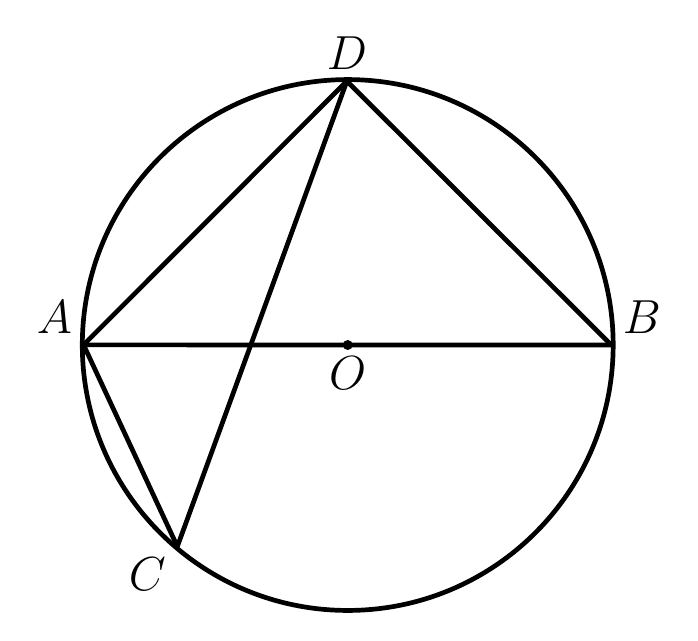
\begin{tikzpicture}[line join=round, line width=1.7pt]
\coordinate (A) at (-3.378,-0.374);
\coordinate (B) at (3.325,-0.377);
\coordinate (C) at (-2.187,-2.935);
\coordinate (D) at (-0.034,2.975);
\coordinate (O) at (-0.023,-0.376);

  
  \draw (O) circle[radius=3.371];
  
  \draw (A) -- (B);
  \draw (A) -- (D);
  \draw (D) -- (B);
  \draw (D) -- (C);
  \draw (A) -- (C);
  
  \fill (O) circle[radius=1.800pt];
  
  \node[above left] at (A) {\fontsize{18}{21.6}\selectfont $A$};
  \node[above right] at (B) {\fontsize{18}{21.6}\selectfont $B$};
  \node[above] at (D) {\fontsize{18}{21.6}\selectfont $D$};
  \node[below left] at (C) {\fontsize{18}{21.6}\selectfont $C$};
  \node[below] at (O) {\fontsize{18}{21.6}\selectfont $O$};
\end{tikzpicture}
\end{document}